\documentclass{article}
\usepackage{graphicx} % Required for inserting images

\title{Assignment 3}
\author{Anagha Samaga}
\date{May 2026}

\maketitle

\section{Question 1:}
In this section, I iterated the function $z_{n+1} = z_n^2 + c$ and the set of all points $c$ in the complex plane for which the sequence remains bounded is in the middle of the plot. The central yellow shade and circular bulbs represent complex points $c$ that are bounded and belong to the set. This was created by creating grid of points representing the complex plane, and for each point \$c\$, the sequence was iterated to determine if it remained bounded. The iteration continued until either the magnitude \$|z|\$ squared exceeded $4$ or a maximum iteration count of 500 was reached. Then, it was plotted using matplotlib. 

\begin{figure}
    \centering
    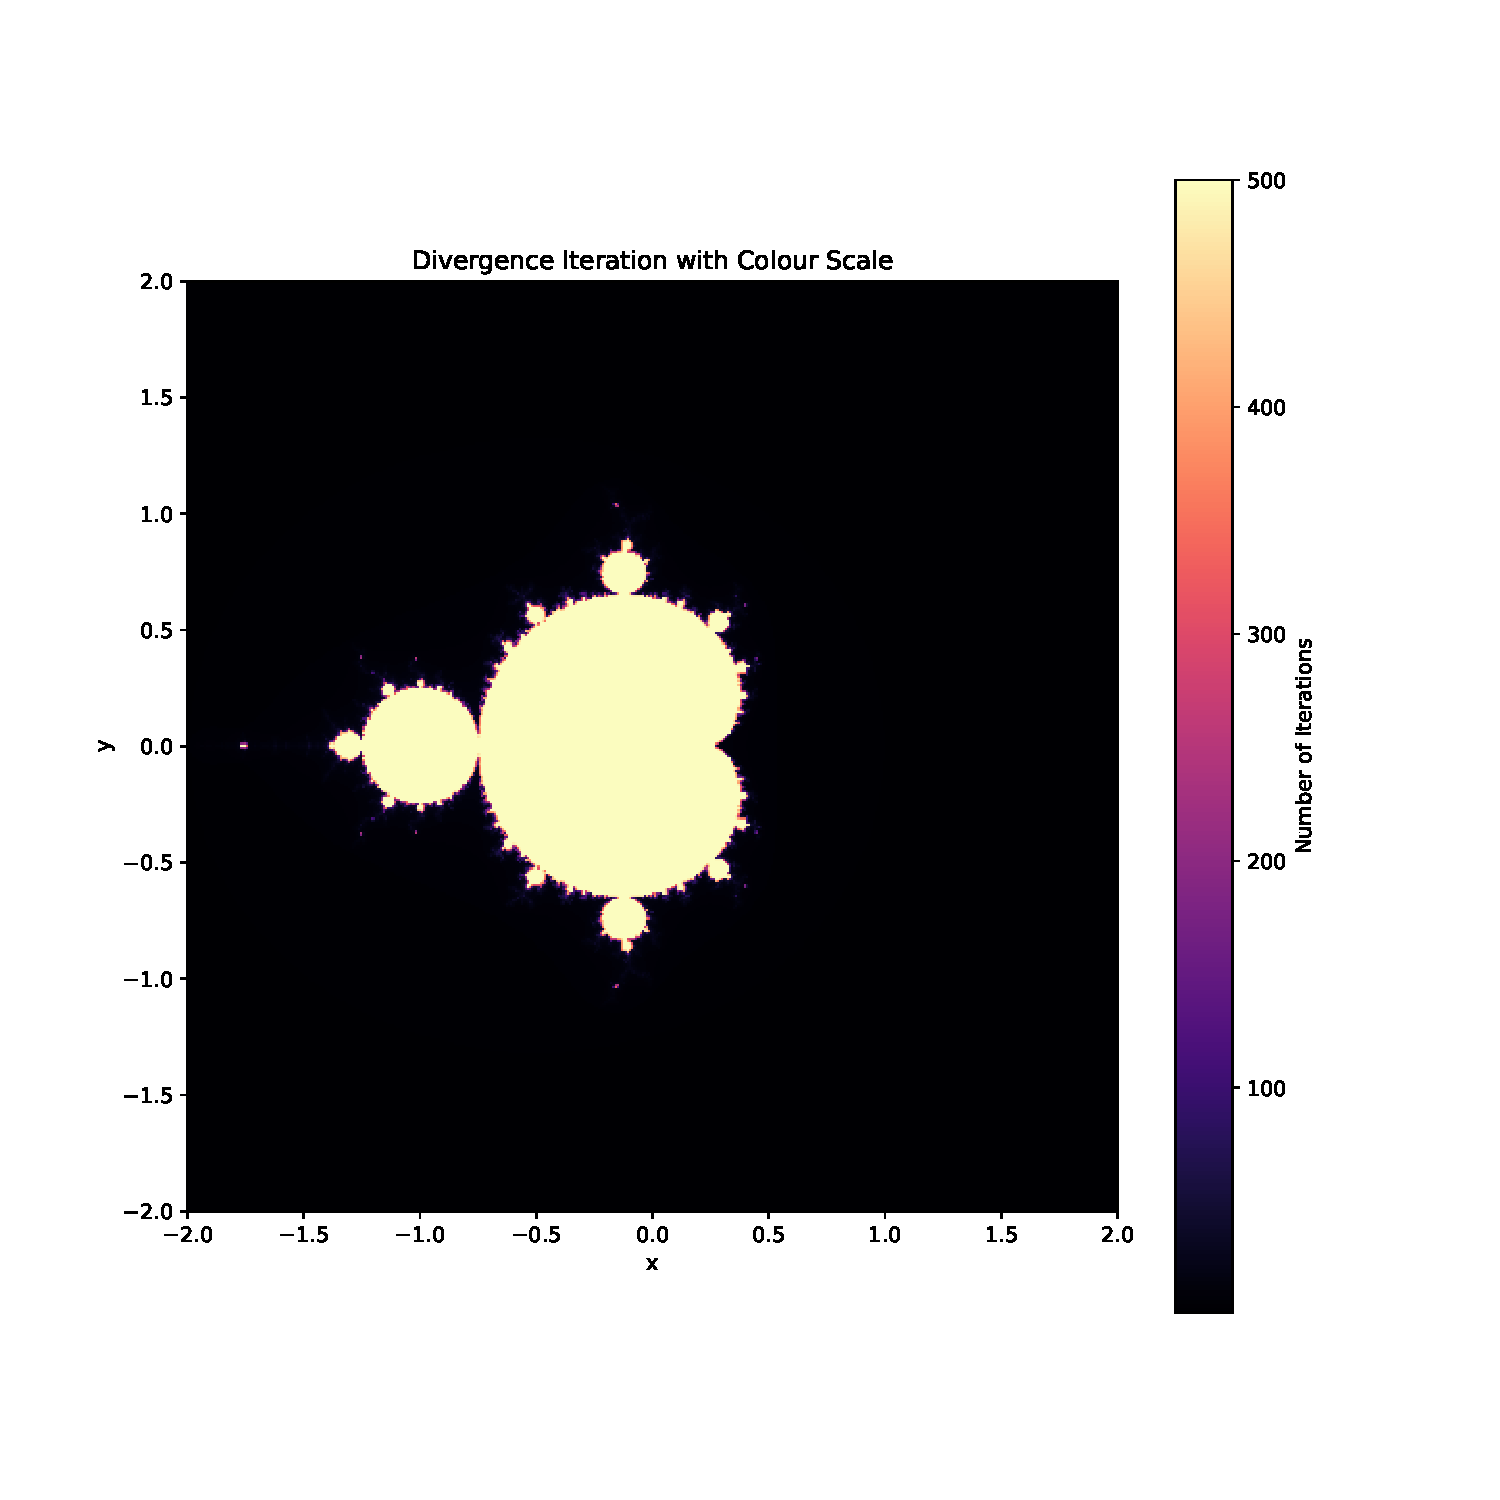
\includegraphics[width=1\linewidth]{colour_scaled_iterations.pdf}
    \caption{The set visualized with a color scale representing the rate of divergence.}
    \label{fig:1}
\end{figure}

\section{Question 2: The Lorenz Equations}

 The following systems were solved using scipy's solve_ivp. 
\begin{equation}
    \dot{X} = -\sigma(X - Y), \quad \dot{Y} = rX - Y - XZ, \quad \dot{Z} = -bZ + XY
\end{equation}
Using the parameters $\sigma=10$, $r=28$, and $b=8/3$.

The system was integrated for dimensionless time units \ $ t=60 \ $ using an ODE solver with the original Lorenz parameter values: $sigma = 10., r = 28. ,$ and $b = 8/3.$. The initial conditions used were $W_0 = [0., 1., 0.]$. Later, to analyze sensitivity, a second integration was performed with a slightly perturbed initial condition, $W'_0 = [0., 1.00000001, 0.]$. 
Figure \ref{fig:2} shows the trajectory in the $Y-Z$ phase plane between $t=14$ and $t=19$.

\begin{figure}[h!]
    \centering
    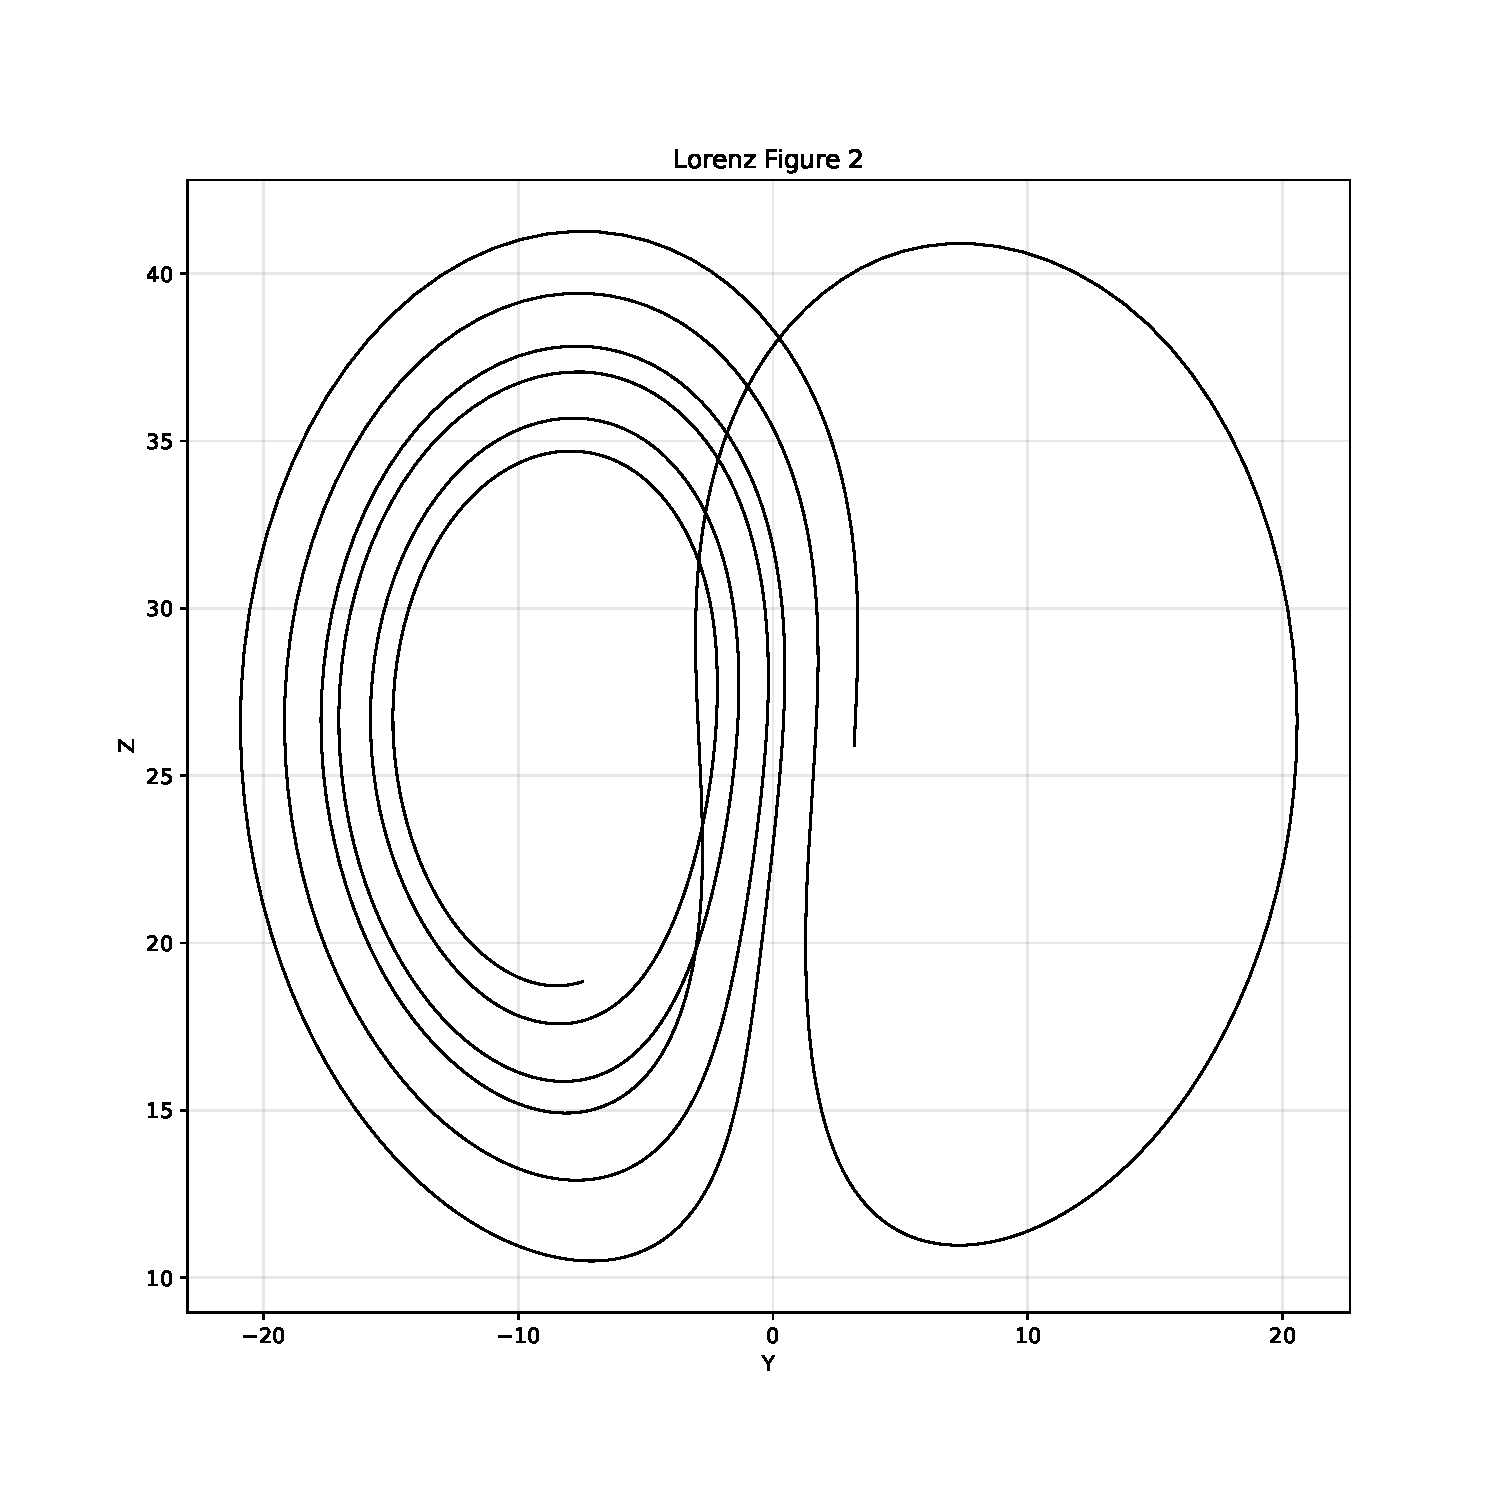
\includegraphics[width=0.8\textwidth]{lorenz_fig2.pdf}
    \caption{Evolution of variable $Y$ against $N = t/0.01$.}
    \label{fig:2}
\end{figure}

\end{document}
